\section{Operazioni sulle Opere}

%%%%%%%%%%%%%%%%%%%%%%%%%%%
%     Visualizza Opera    %
%%%%%%%%%%%%%%%%%%%%%%%%%%%
\subsection{Visualizzazione}
\begin{itemize}
	\item \textbf{Procedure coinvolte}: VisualizzaOpera
	\item \textbf{Obiettivo}: Visualizzare i dettagli e le descrizioni di un'Opera nella base di dati
	\item \textbf{Parametri}:
	\begin{enumerate}
		\item \textbf{operaID}: in NUMBER
		\item \textbf{lingue}: in VARCHAR2, la lingua delle decrizioni da visualizzare
		\item \textbf{livelli}: in VARCHAR2, il livello delle descrizioni da visualizzare
	\end{enumerate}
	\item \textbf{Risultato}: Visualizza l'Opera richiesta, le descrizioni presenti, gli autori, il museo e la sala in cui si trova
	\item \textbf{Usa}: Opere, AutoriOpere, Descrizioni, SaleOpere, Stanze, Sale, Musei, Autori
	\item \textbf{Modifica}: nessuna
	\item \textbf{Precondizioni}:
	\begin{itemize}
		\item $\exists! opera \in Opere : opera.IdOpera = operaID$
	\end{itemize}
	\item \textbf{Postcondizioni}: nessuna
	\item \textbf{Note}:
	Il museo di apparteneza non viene mostrato, se differisce dal museo di esposizione è ricavabile dallo \hyperref[Storico prestiti dell'Opera]{\textbf{Storico prestiti dell'Opera}}.
\end{itemize}

%%%%%%%%%%%%%%%%%%%%%%%%%%%
%     Inserisci Opera     %
%%%%%%%%%%%%%%%%%%%%%%%%%%%
\subsection{Inserimento}
\begin{itemize}
	\item \textbf{Procedure coinvolte}: InserisciOpera, ConfermaDatiOpera, InserisciDatiOpera
	\item \textbf{Obiettivo}: Inserisce una nuova Opera nel database
	\item \textbf{Parametri}:
	\begin{enumerate}
		\item \textbf{Titolo}: in VARCHAR2
		\item \textbf{Anno}: in VARCHAR2
		\item \textbf{FinePeriodo}: in VARCHAR2, \textbf{opzionale}, fine del periodo di realizzazione 
		\item \textbf{IdMusei}: in NUMBER
	\end{enumerate}
	\item \textbf{Risultato}: Inserisce l'Opera richiesta nella base di dati, oppure restituisce un errore
	\item \textbf{Errori}: 
	\begin{itemize}
	%\item L'Opera con i dati inseriti è già presente nel database
		\item Parametri obbligatori con valore nullo (solo se chiamata a ConfermaDatiOpera senza passare da InserisciOpera)
		\item Parametri newAnno e newFineperiodo presentano caratteri non numerici
	\end{itemize}
	\item \textbf{Usa}: Opere, Musei, AppartieneA
	\item \textbf{Modifica}: Opere
	\item \textbf{Precondizioni}:
	\begin{itemize}
		\item $MuseoID \ne null \land Titolo \ne null \land Anno \ne null$
		\item $\exists x \in Musei : x.IdMuseo = MuseoID$
		%\item $\nexists x \in Opere : x.Museo = MuseoID \land x.Titolo = Titolo \land x.Anno = Anno$
		\item $|Opere| = n$
	\end{itemize}
	\item \textbf{Postcondizioni}:
	\begin{itemize}
		\item $\exists! opera \in Opere : opera = (IdOpera.nextval, titolo, anno, fineperiodo, museo, 1, 0)$
	\end{itemize}
\end{itemize}
\clearpage
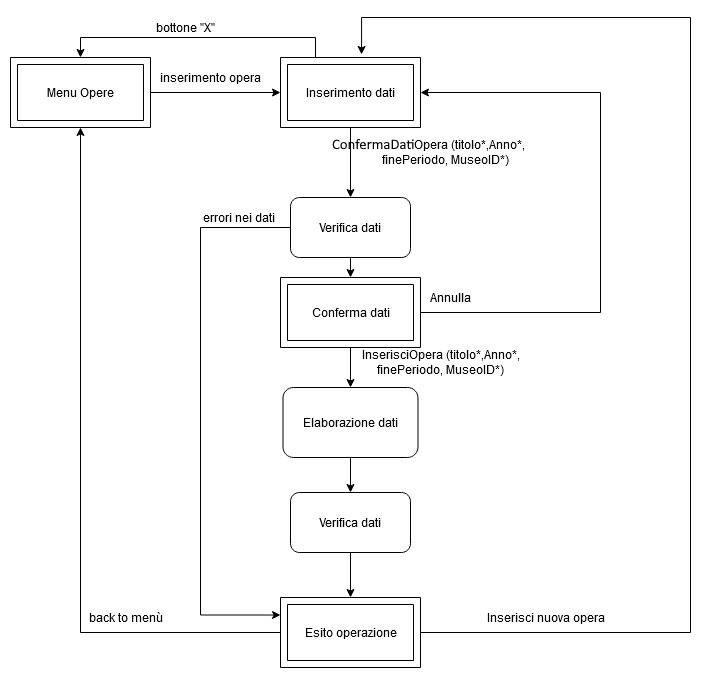
\includegraphics[width=\textwidth]{img/InserimentoOpere.jpg}\\[1cm]

%%%%%%%%%%%%%%%%%%%%%%%%%%%
%     Modifica Opera      %
%%%%%%%%%%%%%%%%%%%%%%%%%%%
\subsection{Modifica}
\begin{itemize}
	\item \textbf{Procedure coinvolte}: ModificaOpera, ConfermaUpdateOpera, UpdateOpera
	\item \textbf{Obiettivo}: Modifica un'Opera presente nel database
	\item \textbf{Parametri}:
	\begin{enumerate}
		\item \textbf{OperaID}: in NUMBER
		\item \textbf{newTitolo}: in VARCHAR2
		\item \textbf{newAnno}: in VARCHAR2
		\item \textbf{newFineperiodo}: in VARCHAR2, opzionale
		\item \textbf{newIdMusei}: in NUMBER
	\end{enumerate}
	\item \textbf{Risultato}: Modifica l'Opera specificata se esiste nella base di dati, errore altrimenti (la base di dati rimane inalterata)
	\item \textbf{Errori}: 
	\begin{itemize}
		\item L'Opera con OperaID non è presente nel database
		\item Parametri obbligatori con valore nullo
		\item Parametri newAnno e newFineperiodo presentano caratteri non numerici
	\end{itemize}
	\item \textbf{Usa}: Opere, Musei
	\item \textbf{Modifica}: Opere
	\item \textbf{Precondizioni}:
	\begin{itemize}
		\item $\exists x \in Opere : x.IdOpera = OperaID$
		\item $newTitolo \ne null \land newAnno \ne null \land newFineperiodo \ne null \land newIdMusei \ne null$
		\item $\exists x \in Musei : x.IdMuseo = newmuseum$
		\item $|Opere| = n$
	\end{itemize}
	\item \textbf{Postcondizioni}: se $x \in Opere \land x.IdOpera = OperaID$
	\begin{itemize}
		\item $x.Titolo := newtitle$
		\item $x.Anno := newyear$
		\item $x.Fineperiodo := newFinePeriodo$
		\item $x.Museo := newIdMusei$
		\item $|Opere| = n$
	\end{itemize}
	\item \textbf{Note}:
	%% TODO: add link aggiungiAutore/rimuoviAutore
	Nel form di modifica è possibile anche aggiungere o rimuovere autori, se autorizzati.
	Per realizzare tale operazione viene richiamata la procedura \hyperref[AggiuntaAutore]{\textbf{Aggiunta autore}}
	o \hyperref[RimozioneAutoreOpera]{\textbf{Rimozione autore}} e poi si è rediretti al
	menu delle opere al termine dell'operazione
\end{itemize}
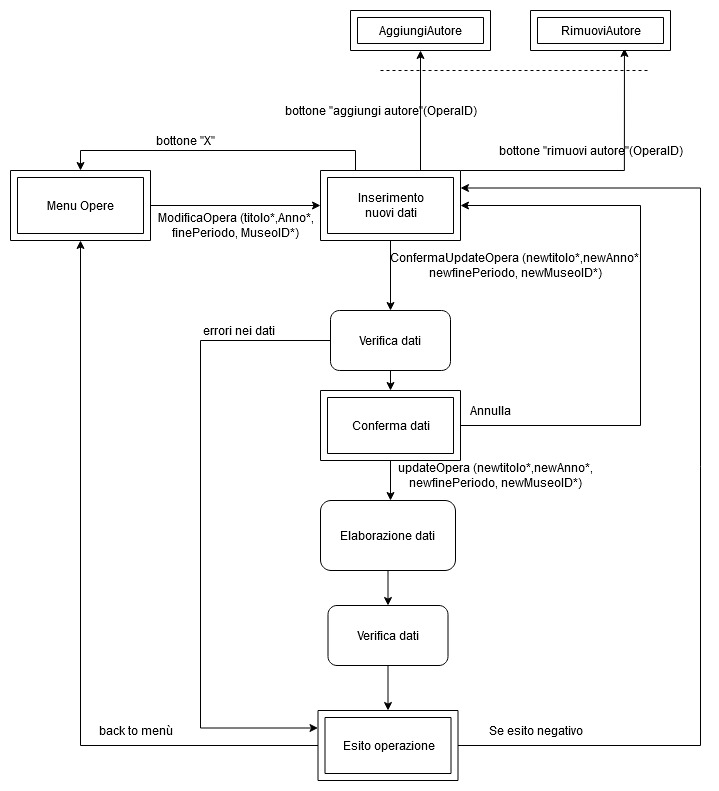
\includegraphics[width=\textwidth]{img/UpdateOpera.jpg}\\[1cm]


%%%%%%%%%%%%%%%%%%%%%%%%%%%
%     Elimina Opera       %
%%%%%%%%%%%%%%%%%%%%%%%%%%%
\subsection{Eliminazione}
\begin{itemize}
	\item \textbf{Procedure coinvolte}: EliminazioneOpera, RimozioneOpera
	\item \textbf{Obiettivo}: Elimina un'opera dalla lista di quelle visibili agli Utenti, senza rimuoverla dal database
	\item \textbf{Parametri}:
	\begin{enumerate}
		\item \textbf{OperaID}: in NUMBER
	\end{enumerate}
	\item \textbf{Risultato}: L'opera individuata da operaID viene resa non visibile agli utenti, ma se e solo se non è al momento esposta in alcun museo. Se lo è l'eliminazione non è concessa e la base di dati non è alterata
	\item \textbf{Errori}: 
	\begin{itemize}
		\item L'Opera individuata da operaID è in esposizione in un museo
		\item L'Opera con OperaID non è presente nel database
	\end{itemize}
	\item \textbf{Usa}: Opere, SaleOpere, AutoriOpere, Descrizioni
	\item \textbf{Modifica}: Opere
	\item \textbf{Precondizioni}:
	\begin{itemize}
		\item $\exists x \in Opere : x.IdOpera = OperaID$
		\item $\nexists x \in SaleOpere : x.Opera=operaID \land x.DataUscita = null$
	\end{itemize}
	\item \textbf{Postcondizioni}:
	\begin{itemize}
		\item $\exists x \in Opere : x.IdOpera = operaID \land x.Eliminato = 1$
	\end{itemize}
	%% TODO: controllare semantica
	\item \textbf{Note}: Le informazioni correlate all'opera non sono alterate
\end{itemize}

%%%%%%%%%%%%%%%%%%%%%%%%%%%
%     Rimuovi Opera       %
%%%%%%%%%%%%%%%%%%%%%%%%%%%
\subsection{Rimozione}
\begin{itemize}
	\item \textbf{Procedure coinvolte}: EliminazioneDefinitivaOpera, RimozioneDefinitivaOpera
	\item \textbf{Obiettivo}: Rimuove un'Opera dal database
	\item \textbf{Parametri}:
	\begin{enumerate}
		\item \textbf{OperaID}: in NUMBER
	\end{enumerate}
	\item \textbf{Risultato}: L'opera individuata da operaID viene rimossa dalla base di dati
	\item \textbf{Errori}: 
	\begin{itemize}
		\item L'Opera individuata da operaID è in esposizione in un museo
		\item L'Opera con OperaID non è presente nel database
	\end{itemize}
	\item \textbf{Usa}: Opere, SaleOpere, AutoriOpere, Descrizioni
	\item \textbf{Modifica}: Opere, SaleOpere, AutoriOpere, Descrizioni
	\item \textbf{Precondizioni}:
	\begin{itemize}
		\item $\exists x \in Opere : x.IdOpera = OperaID$
		\item $\nexists x \in SaleOpere : x.Opera=operaID \land x.DataUscita = null$
	\end{itemize}
	\item \textbf{Postcondizioni}:
	\begin{itemize}
		\item $\nexists x \in Opere : x.IdOpera = operaID$
	\end{itemize}
	%% TODO: controllare semantica
	\item \textbf{Note}: Tutte le tracce dell'opera dalle tabelle modificate sono rimosse
\end{itemize}

%%%%%%%%%%%%%%%%%%%%%%%%%%%
%  Aggiunta Autore Opera  %
%%%%%%%%%%%%%%%%%%%%%%%%%%%
% Si intende l'aggiunta di un autore già esistente nella base di dati
\label{AggiuntaAutore}
\begin{itemize}
	\item \textbf{Procedure coinvolte}: AggiungiAutore
	\item \textbf{Obiettivo}: Aggiunge un Autore ad un'Opera, se entrambe le entità sono presenti nella base di dati
	\item \textbf{Parametri}:
	\begin{enumerate}
		\item \textbf{OperaID}: in NUMBER
		\item \textbf{AutoreID}: in NUMBER
		\item \textbf{lingue}: in VARCHAR2, opzionale, per redirect alla visualizzazione
	\end{enumerate}
	\item \textbf{Risultato}: Aggiunge l'autore con l'ID indicato all'Opera individuata dall'ID dato.\\
	Se l'autore specificato compare già tra gli autori dell'Opera, allora la base di dati rimane inalterata
	\item \textbf{Errori}: 
	\begin{itemize}
		\item L'autore individuato da AuthorID è già stato aggiunto come autore di quest'Opera
	\end{itemize}
	\item \textbf{Usa}: Autori, AutoriOpere
	\item \textbf{Modifica}: AutoriOpere
	\item \textbf{Precondizioni}:
	\begin{itemize}
		\item $\exists x \in Opere : x.IdOpera = OperaID$
		\item $\exists y \in Autori : y.IdAutore = AuthorID$
		\item $\nexists z \in AutoriOpere : z.IdAutore = AuthorID \land z.IdOpera = OperaID$
		\item $|AutoriOpere| = n$
	\end{itemize}
	\item \textbf{Postcondizioni}:
	\begin{itemize}
		\item $\exists z \in AutoriOpere : z.IdAutore = AuthorID \land z.IdOpera = OperaID$
		\item $|AutoriOpere| = n + 1$
	\end{itemize}
\end{itemize}
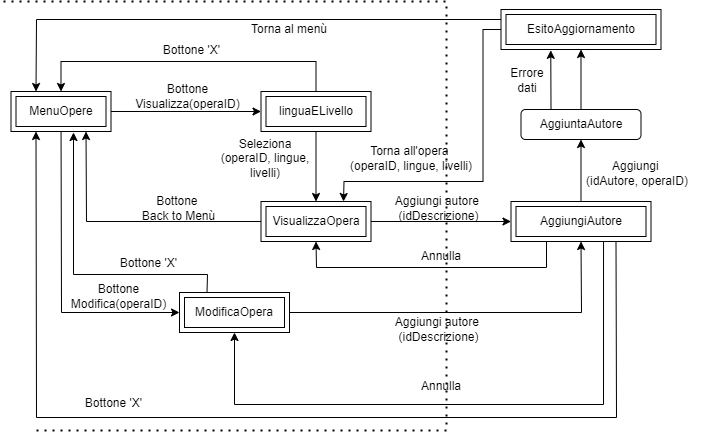
\includegraphics[width=\textwidth]{img/AggiungiAutore.png}

\label{RimozioneAutoreOpera}
\subsection{Rimozione Autore Opera}
\begin{itemize}
	\item \textbf{Procedure coinvolte}: RimozioneAutoreOpera, RimuoviAutoreOpera
	\item \textbf{Obiettivo}: Rimuove un Autore da un'Opera, se entrambe le entità sono presenti nella base di dati ed è presente l'associazione tra autore ed opera
	\item \textbf{Parametri}:
	\begin{enumerate}
		\item \textbf{OperaID}: in NUMBER
		\item \textbf{AutoreID}: in NUMBER
		\item \textbf{lingue}: in VARCHAR2, opzionale, per redirezione verso visualizzazione opera
	\end{enumerate}
	\item \textbf{Risultato}: Rimuove l'autore con l'ID indicato dall'Opera individuata dall'ID dato.\\
	Se l'autore specificato non compare già tra gli autori dell'Opera, allora la base di dati rimane inalterata
	\item \textbf{Errori}:
	\begin{itemize}
		\item L'autore individuato da AuthorID non è associato all'opera individuata da OperaID
	\end{itemize}
	\item \textbf{Usa}: Autori, AutoriOpere
	\item \textbf{Modifica}: AutoriOpere
	\item \textbf{Precondizioni}:
	\begin{itemize}
		\item $\exists x \in Opere : x.IdOpera = OperaID$
		\item $\exists y \in Autori : y.IdAutore = AuthorID$
		\item $\exists z \in AutoriOpere : z.IdAutore = AuthorID \land z.IdOpera = OperaID$
		\item $|AutoriOpere| = n$
	\end{itemize}
	\item \textbf{Postcondizioni}:
	\begin{itemize}
		\item $\nexists z \in AutoriOpere : z.IdAutore = AuthorID \land z.IdOpera = OperaID$
		\item $|AutoriOpere| = n - 1$\\
	\end{itemize}
	\item \textbf{Note}: il diagramma di flusso è analogo a quello della rimozione, per cui abbiamo ritenuto superfluo inserirlo anche per questa operazione
\end{itemize}

\label{Filtraggio delle opere}
\subsection{Filtraggio delle Opere}
\begin{itemize}
	\item \textbf{Procedure coinvolte}: menuOpere(o menuOpereEliminate), filtraOpere
	\item \textbf{Obiettivo}: mostrare determinate opere in base a dei filtri selezionabili dagli utenti in filtraOpere
	\item \textbf{Parametri}:
	\begin{enumerate}
		\item \textbf{orderBy}: in VARCHAR2
		\item \textbf{nameFilter}: in VARCHAR2
		\item \textbf{MuseoFilter}: in NUMBER
		\item \textbf{AutoriFilter}: in NUMBER 
		\item \textbf{AnnoFilterInizio}: in NUMBER 
		\item \textbf{AnnoFilterFine}: in NUMBER
	\end{enumerate}
	\item \textbf{Risultato}: Mostra in menuOpere(o in menuOpereEliminate) le opere che rispettano i filtri selezionati. In caso non siano stati selezionati filtri vengono mostrate tutte le opere in ordine alfabetico
	\item \textbf{Usa}: Autori, AutoriOpere, Opere
	\item \textbf{Modifica}: niente
\end{itemize}

\subsection{Statistiche e monitoraggio}
Il diagramma riportato di seguito è valido per tutte le statistiche relative alle opere, dato che rappresenta il flusso di informazioni per ciascuna delle scelte dal popup di selezione.\\[1cm]
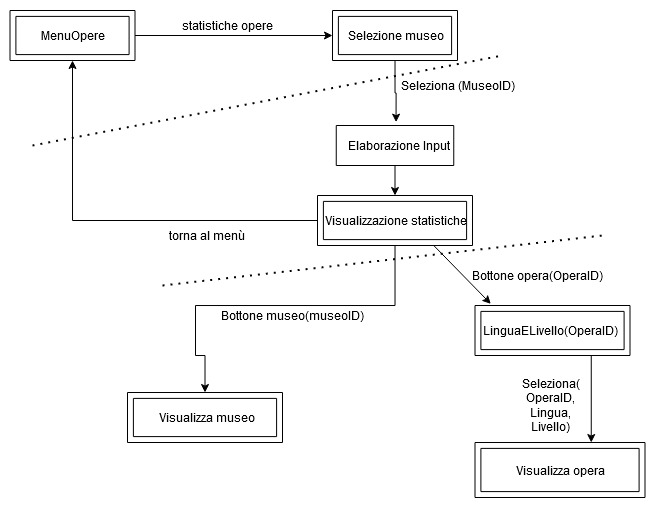
\includegraphics[width=\textwidth]{img/VisualizzazioneStatistiche.jpg}\\[1cm]

\subsubsection{Storico prestiti dell’Opera}
\begin{itemize}
    \item \textbf{Procedure Coinvolte}: SpostamentiOpera
    \item \textbf{Obiettivo}: Mostrare lo storico dei prestiti di una determinata opera
    \item \textbf{Parametri}:
	\begin{enumerate}
		\item \textbf{OperaID}: in NUMBER
	\end{enumerate}
	\item \textbf{Risultato}: Mostra il proprietario, il destinatario e il periodo del prestito
	\item \textbf{Usa}: Musei, SaleOpere, Opere, Stanze
	\item \textbf{Modifica}: niente
	\item \textbf{Precondizioni}:
	\begin{itemize}
		\item $\exists x \in Opere : x.IdOpera = OperaID$
		\item $\exists y \in SaleOpera : y.opera = operaID$
		\item $\exists z \in SaleOpere : \exists w \in Stanze : z.idStanza = w.sala \land w.Opera = OperaID$
	\end{itemize}
	\item \textbf{Postcondizioni}: nessuna
\end{itemize}
%\subsubsection{Autori dell’Opera}
%\subsubsection{Tipo Sala in cui si trova l’Opera}
%\subsubsection{Descrizioni dell’Opera}

\subsubsection{Lista Opere ordinate per numero di Autori in ordine decrescente}
\begin{itemize}
	\item \textbf{Procedure coinvolte}: statisticheOpere, menuOpere, selezioneMuseo
	\item \textbf{Obiettivo}: Mostra le opere con il maggior numero di autori
	\item \textbf{Parametri}:
	\begin{enumerate}
		\item \textbf{museoID}: in NUMBER
	\end{enumerate}
	\item \textbf{Risultato}: Mostra il nome delle prime tre opere, se museoID $\neq 0$ relative a quel museo altrimenti tra tutti i musei, con il maggior numero di autori e il numero di autori dell'opera
	\item \textbf{Errori}: nessuno
	\item \textbf{Usa}: Opere, AutoriOpere, Musei
	\item \textbf{Modifica}: niente
	\item \textbf{Precondizioni}:
	\begin{itemize}
		\item $|opere| \ge 3$
	\end{itemize}
	\item \textbf{Postcondizioni}: nessuna
\end{itemize}

\subsubsection{Opere non spostata da più tempo (le tre più vecchie)}
\begin{itemize}
	\item \textbf{Procedure coinvolte}: statisticheOpere, menuOpere, selezioneMuseo
	\item \textbf{Obiettivo}: Mostra le opere non spostate da più tempo
	\item \textbf{Parametri}:
	\begin{enumerate}
		\item \textbf{museoID}: in NUMBER
	\end{enumerate}
	\item \textbf{Risultato}: Mostra il nome delle prime tre opere, se museoID $\neq 0$ relative a quel museo altrimenti tra tutti i musei, non spostate da più tempo e per quanti giorni non sono state spostate
	\item \textbf{Errori}: nessuno
	\item \textbf{Usa}: Opere, saleOpere, Musei
	\item \textbf{Modifica}: niente
	\item \textbf{Precondizioni}:
	\begin{itemize}
		\item $|opere| \ge 3$
	\end{itemize}
	\item \textbf{Postcondizioni}: nessuna
\end{itemize}

\subsubsection{Opere esposte per più tempo (le tre più vecchie)}
\begin{itemize}
	\item \textbf{Procedure coinvolte}: statisticheOpere, menuOpere, selezioneMuseo
	\item \textbf{Obiettivo}: Mostra le opere esposte per più tempo
	\item \textbf{Parametri}:
	\begin{enumerate}
		\item \textbf{museoID}: in NUMBER
	\end{enumerate}
	\item \textbf{Risultato}: Mostra il nome delle prime tre opere, se museoID $\neq 0$ relative a quel museo altrimenti tra tutti i musei, esposte da più tempo e per quanti giorni sono state esposte
	\item \textbf{Errori}: nessuno
	\item \textbf{Usa}: Opere, saleOpere, Musei
	\item \textbf{Modifica}: niente
	\item \textbf{Precondizioni}:
	\begin{itemize}
		\item $|opere| \ge 3$ 
	\end{itemize}
	\item \textbf{Postcondizioni}: nessuna
\end{itemize}
%\subsubsection{Età media delle opere}

\subsubsection{Ordinamento per anno di realizzazione (le tre più vecchie)}
\begin{itemize}
	\item \textbf{Procedure coinvolte}: statisticheOpere, menuOpere, selezioneMuseo
	\item \textbf{Obiettivo}: Mostra le opere più antiche
	\item \textbf{Parametri}:
	\begin{enumerate}
		\item \textbf{museoID}: in NUMBER
	\end{enumerate}
	\item \textbf{Risultato}: Mostra il nome delle prime tre opere, se museoID $\neq 0$ relative a quel museo altrimenti tra tutti i musei, più antiche e l'età, in anni, dell'opera
	\item \textbf{Errori}: nessuno
	\item \textbf{Usa}: Opere, Musei
	\item \textbf{Modifica}: niente
	\item \textbf{Precondizioni}:
	\begin{itemize}
		\item $|opere| \ge 3$
	\end{itemize}
	\item \textbf{Postcondizioni}: nessuna
\end{itemize}
